\documentclass[a4paper]{article}
\usepackage[14pt]{extsizes}
\usepackage[utf8]{inputenc}
\usepackage[russian]{babel}
\usepackage{setspace,amsmath}
\usepackage[left=20mm, top=15mm, right=15mm, bottom=15mm, nohead, footskip=10mm]{geometry}
\usepackage{hyperref}
\hypersetup{
    colorlinks,
    citecolor=black,
    filecolor=black,
    linkcolor=black,
    urlcolor=black
}
\usepackage{graphicx}
\graphicspath{{./}}
\graphicspath{{./pictures/}}
\DeclareGraphicsExtensions{.pdf,.png,.jpg}
\usepackage[tableposition=top,singlelinecheck=false]{caption}
\usepackage{subcaption}
\DeclareCaptionLabelFormat{gostfigure}{Рисунок #2}
\captionsetup*[figure]{labelformat=gostfigure, justification=centering}
\usepackage{amsfonts}

\begin{document}
 
\begin{center}

\includegraphics{MSU}

\hfill \break
\normalsize{Московский государственный университет имени М.В. Ломоносова}\\
\normalsize{Факультет вычислительной математики и кибернетики}\\
\normalsize{Кафедра информационной безопаснсти}\\
\normalsize{Лаборатория безопасности информационных систем}\\
 \hfill \break
\normalsize{Николайчук Артём Константинович}\\
\hfill\break
\hfill \break
\hfill \break
\hfill \break
\large{Обзор методов тестирования zk circuits для проверки полноты их ограничений}\\
\hfill \break
\hfill \break
\hfill \break
\normalsize{Курсовая работа}\\
\hfill \break
\hfill \break
\hfill \break
\hfill \break
\hfill \break
\hfill \break
\hfill \break
\hfill \break
\begin{flushright}
    \normalsize{Научный руководитель:}\\
    \normalsize{программист кафедры ИБ}\\
    \normalsize{М.С.Воронов}\\
\end{flushright}
\end{center}
\vspace*{\fill}
\begin{center} Москва, 2024 \end{center}
\thispagestyle{empty}
 
\newpage
\section*{Аннотация}
\indent

В настоящее время всё большую популярность получают решения второго уровня(L2) на блокчейне. L2 уровень на блокчейне обозначает второй уровень масштабируемости и решает проблемы масштабирования и скорости транзакций, которые могут возникать на первом уровне блокчейна (L1).
L2 может быть представлен различными протоколами, такими как Lightning Network для биткоина или Polygon для Ethereum. Эти протоколы позволяют совершать децентрализованные транзакции и выполнять смарт-контракты вне цепи блоков, что уменьшает нагрузку на основную сеть и повышает ее масштабируемость. L2 уровень также обеспечивает более быстрые и дешевые транзакции, что делает использование блокчейна более удобным и доступным для всех участников сети. В таких протоколах часто используют zk circuit - схемы, которые позволяют доказывать, что какие-то действия были выполнены пользователем, например что пользователь совершил транзакцию токена со своего аккаунта, либо то, что пользователь знает какой-то определённый секрет. Цена ошибки или бага в таких схемах может быть невероятно высокой - потенциальные уязвимости могут быть использованы для кражи всех токенов протокола. Допустить ошибку при разработке легко - иногда достаточно забыть добавить одно условие. Для поиска недостаточно ограниченных схем разумно применять методы автоматического тестирования. Такие методы рассматриваются в этой работе.

\newpage
    \tableofcontents
\newpage
 
\newpage
\section{Введение}

\subsection{zk-rollups}
\indent

Описание на примере блокчейна Эфириум. ZK-rollup - это протокол вне основной сети, который работает поверх блокчейна Ethereum и управляется встроенными смарт-контрактами Ethereum. ZK-rollup выполняет транзакции за пределами основной сети, но периодически передает пакеты транзакций вне сети в сетевой накопительный контракт. Эта запись транзакции является неизменяемой, как и в блокчейне Ethereum, и формирует цепочку ZK-rollup.

Базовая архитектура ZK-rollup представлена на рисунке \ref{ZK-rollup} и состоит из следующих компонентов:

\begin{figure}[ht!]
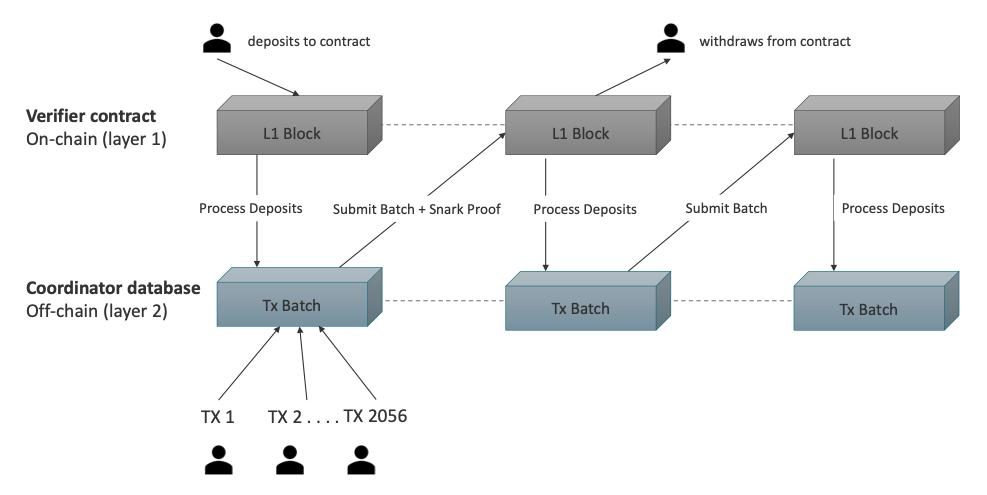
\includegraphics[width=180mm]{Layer-2-architecture.jpg}
\caption{Архитектура ZK-rollup}
\label{ZK-rollup}
\end{figure}

\begin{itemize}
\item Сетевые контракты. Протокол ZK-rollup управляется смарт-контрактами, работающими на Ethereum. Это включает в себя основной контракт, который хранит накопительные блоки, отслеживает депозиты и отслеживает обновления состояния. Другой сетевой контракт (verifier contract) проверяет доказательства с нулевым разглашением, представленные производителями блоков. Таким образом, Ethereum служит базовым уровнем или "L1" для ZK-rollup.

\item Автономная виртуальная машина (ВМ). В то время как протокол ZK-rollup работает в Ethereum, выполнение транзакций и хранение состояния происходит на отдельной виртуальной машине. Эта автономная виртуальная машина является средой выполнения транзакций в ZK-rollup и служит в качестве дополнительного уровня или "L2" для протокола ZK-rollup. Доказательства достоверности, проверенные в сети Ethereum, гарантируют корректность перехода состояний в автономной виртуальной машине.
\end{itemize}

Состояние ZK-rollup, включающее счета и балансы L2, представлено в виде дерева Меркла. Криптографический хэш корня дерева Меркла хранится в контракте основного блокчейна, позволяя протоколу rollup отслеживать изменения в состоянии ZK-rollup.

Оператор(L2), инициировавший переход в другое состояние, должен вычислить новый корневой код состояния и выполнить отправку по цепочке контрактов. Помимо самого состояния оператов генерирует доказательство, которое подтверждает, что все переходы были легитимными и новый корень дерева Меркла действителен. Если подтверждение достоверности, связанное с пакетом, аутентифицируется контрактом верификации, новый корень дерева становится корнем канонического состояния ZK-rollup. Именно тут открываются большие возможности для злоумышленников в случае ошибки в схеме доказательста.

Помимо вычисления корней состояний, оператор ZK-rollup также создает пакетный корень — корень дерева Меркла, содержащий все транзакции в пакете. При отправке нового батча в сводном контракте сохраняется корень пакета, что позволяет пользователям подтвердить, что транзакция (например, запрос на вывод средств) была включена в пакет. Пользователи должны будут предоставить информацию о транзакции, корень пакета и подтверждение Merkle, показывающее путь включения.

\subsection{Деревья Меркла}
\indent

Деревья Меркла - это особый вариант древовидной структуры данных, в котором новые данные вставляются в виде листа в нижней части дерева и для каждого уровня пары из двух листьев хэшируются вместе. Соответственно, количество узлов уменьшается вдвое на каждом новом уровне, пока не останется один с единственным хэшем, корневым хэшем дерева Меркле.

Иллюстрация базового дерева Меркле с восемью элементами данных представлена на рисунке \ref{Merkle_tree}

\begin{figure}[ht!]
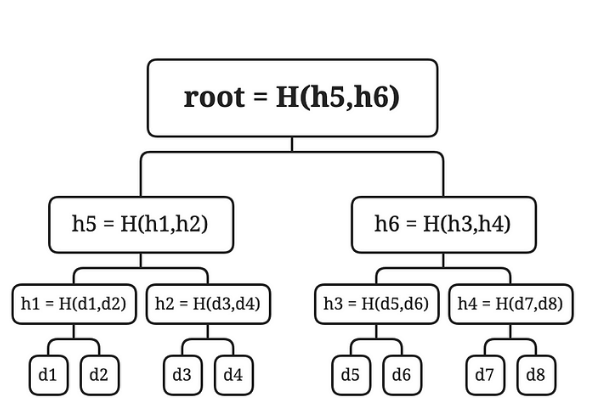
\includegraphics[width=180mm]{Merkle_tree.png}
\caption{Пример дерева Меркла}
\label{Merkle_tree}
\end{figure}

Эта структура данных особенна важна для ZK-rollup, потому что именно она используется для хранения состояния в основной сети. И для доказательства корректности перехода в новое состояние используются различные реализации этих деревьев. Отличительной особенностью реализаций является использование специфичных хеш-функций, таких как Poseidon-hash.\footnote[1]{\href{https://www.poseidon-hash.info/}{https://www.poseidon-hash.info/}}

\subsection{Схемы арифметизации}
\indent

Как отмечено ранее, очень важный шаг перехода в новое состояние на L1 уровне это верификация того, что новый корень дерева Меркла создан корректно. Для создания и проверки этого доказательства используются различные протоколы ZK-SNARKs. Отличительной особенностью таких протоколов являтется то, что они создают короткие доказательства(несколько сотен байт), которые быстро проверяются контрактом в основной сети. Общая схема работы таких протоколов представлена на рисунке \ref{ZK_snark_arch}. Ключевым свойством протоколов zk-snark является то, что подходящее средство доказательства и верификации может быть автоматически сгенерировано из арифметической схемы, представляющей некоторые вычисления. Арифметическая схема принимает некоторые входные сигналы, которые являются значениями в диапазоне $[0, p)$, и выполняет сложение и умножение по модулю простого числа $p$. В результате каждого сложения и умножения генерируется сигнал: промежуточный сигнал от нескольких промежуточных операций и выходной сигнал от конечной операции. В частности, для конкретной арифметической схемы, компиляторы SNARK создают средство доказательства и верификации, преобразуя схему в набор полиномиальных уравнений. Арифметизация - процесс создания генерации схемы по программе. Чтобы упростить этот процесс, криптографическое сообщество разработало такие языки, как Circom\footnote[1]{\href{https://docs.circom.io/}{https://docs.circom.io/}}, Zokrates \footnote[2]{\href{https://zokrates.github.io/}{https://zokrates.github.io/}}, Halo 2 \footnote[3]{\href{https://zcash.github.io/halo2/index.html}{https://zcash.github.io/halo2/index.html}} и другие, которые позволяют пользователям выражать свои предполагаемые вычисления естественным образом.

\begin{figure}[!htb]
    \begin{subfigure}{0.48\linewidth}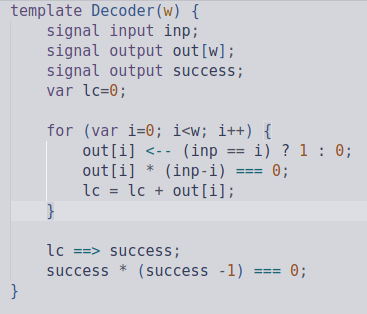
\includegraphics[width=0.88\textwidth]{circom_example_code.png}
    \end{subfigure}
    \begin{subfigure}{0.48\linewidth}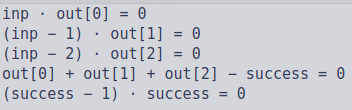
\includegraphics[width=0.88\textwidth]{r1cs_example.png}
    \end{subfigure}
    \caption{Пример программы на языке circom и соответствующая ей схема R1CS}
    \label{broken_example}
 \end{figure}

\subsubsection{R1CS}
\indent
R1CS(Rank 1 Constraint System) - схема арифметизации, которая представляет из себя набор полиномов над полем $F_p$, где $p$ - большое простое число. Система содержит n переменных - это все сигналы, используемые в программе. При этом каждое ограничение(каждый полином) должны быть квадратичными, линейными или постоянными уравнениями
\[
    \begin{cases} 
    (a_{11}*s_1 + ... + a_{1n}*s_n)*(b_{11}*s_1 + ... + b_{1n}*s_n) + (c_{11}*s_1 + ... + c_{1n}*s_n) = 0\\
    (a_{21}*s_1 + ... + a_{2n}*s_n)*(b_{21}*s_1 + ... + b_{2n}*s_n) + (c_{21}*s_1 + ... + c_{2n}*s_n) = 0\\
    (a_{31}*s_1 + ... + a_{3n}*s_n)*(b_{31}*s_1 + ... + b_{3n}*s_n) + (c_{31}*s_1 + ... + c_{3n}*s_n) = 0\\
    ...\\
    (a_{m1}*s_1 + ... + a_{mn}*s_n)*(b_{m1}*s_1 + ... + b_{mn}*s_n) + (c_{m1}*s_1 + ... + c_{mn}*s_n) = 0\\
    \end{cases}
\]

Пример арифметизации для программы на языке circom представлен на рисунке \ref{broken_example}

\subsubsection{Plonkish}
\indent

Plonk(Permutations over Lagrange-bases for
Oecumenical Noninteractive arguments of
Knowledge) арифметизация представляет из себя таблицу со значениями из конечного поля $F_p$. Элементы таблицы называются ячейками. Схемы состоят из элементов управления, которые являются ограничениями, применяемыми к вложенным таблицам (набору ячеек) в таблице. Столбцы таблицы делятся на три основных типа: instance, advice и fixed.
Столбцы Instance хранят общедоступные входные данные, столбцы advice хранят частные секретные данные(witness в общей терминологии) (частные входные данные и промежуточные значения, используемые проверяющим в схеме), а столбцы fixed хранят фиксированные значения, которые являются частью описания схемы. Для этого типа арифметизации используются ограничения на значения в таблице в виде полиномов(гейты) $(q_L)a+(q_R)b+(q_O)c+(q_M)ab+(q_C)=0$. Гейты - это общие полиномиальные ограничения, определенные разработчиком схемы. Каждое такое ограничение применяется к ряду соседних строк логического элемента. Следовательно, схема, табличное представление которой содержит несколько строк, может иметь несколько полиномиальных ограничений, все из которых должны выполняться одновременно. Другой тип ограничений - ограничения на равенство (также известные как ограничения на перестановку или ограничения на копирование) могут заставить определенную группу ячеек иметь одинаковые значения в строках и столбцах.
Таблица и соответствующая её система ограничений - это и есть арифметизация Plonkish.
В Halo2 элементы управления активируются с помощью переменных селекторов. Селектор - это двоичная
переменная, которая умножается на полиномиальное ограничение для каждой строки: оно равно 0, если элемент управления выключен, или 1, если он включен.
Ограничений в виде многочлена выполнено, если его значение равно 0 во всех строках. Все полиномиальные ограничения в системе проверки должны исчезать во всех строках для получения действительной пары секретных и общедоступных входных данных.
Это делается либо путем установки несущественных переменных селектора в 0, либо путем предоставления (возможно, секретных) назначений ячейкам таблицы, которые приводят к вычислению полинома равным 0.

\begin{figure}[ht!]
    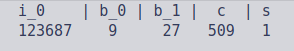
\includegraphics[width=180mm]{plonkish_example.png}
    \caption{Пример арифметизации plonkish}
    \label{plonkish_example}
    \end{figure}

Пример таблицы продемонстрирован на рисунке \ref{plonkish_example}. Здесь $i_0$ - публичная входная переменная, $b_0, b_1$ - секретные переменные, $c$ - константа, $s$ - селектор. Соответствующее ограничение в виде полинома - $s \cdot (c \cdot b_0 \cdot b_1 - i_0) = 0$. То есть схема будет верна только, если доказывающий знает какое-то разложение числа на множители.

\newpage
\section{Цель работы}
\indent

Цель данной работы - сделать обзор методов и средств, используемых при автоматическом тестировании схем арифметизации. Для достижения этой цели требуется:

\begin{itemize}
\item Сформировать критерии для сравнения методов.
\item Проанализировать существующие решения по выделенным критериям.
\item Дать оценку каждому критерию.
\end{itemize}

\newpage
\section{Анализ предметной области}
\indent

\subsection{Уязвимости в схемах арифметизации}
 
Общая черта всех схем арифметизации - наличие ограничений, которые должны выполняться в том случае, если известны все входные параметры - и приватные и публичные. Схемы пишутся на разных специфичных языках программирования(DSL), а затем преобразуются компилятором в один из перечисленных ранее форматов. Объект тестирования - схема в формате R1CS или Plonkish. При разработке схемы или её компилировании могут быть допущены различные ошибки. Например, в схеме может быть целочисленное переполнение - это довольно частая ошибка, потому что разработчики забывают, что все вычисления ведутся в поле $F_p$, или ошибочное использование операторов в программе - например, использование оператора $<--$ вместо $<==$ в Circom. Такие ошибки приводят к тому, что в схеме может быть недостаточно ограничений, то есть для каких-то входных данных может быть несколько корректных секретных данных, что может привести к возможности подмены доказательства. Помимо ошибок при разработке, могут быть ошибке непосредственно в дизайне самой схемы. То есть написанный код будет корректен с точки зрения ЯП и компилятора, но схема будет уязвимой из-за неправильных математических предположений. Далее более формально опишем такие схемы.

Пусть на вход дана арифметическая схема $C(x,y)$. Она является недостаточно ограниченной, если существуют такие публичные входные данные $x$ и два различных выхода $y, y'$ такие, что $C(x, y)$ и $C(x, y')$ оба верны. Вообще говоря, недостаточно ограниченные программы зачастую проблематичны, поскольку они указывают на несоответствие программы по генерации непубличных данных и соответствующих ограничений. В частности, если вычисление является детерминированным, то учитывая вклад $x, y$, есть только один такой $y$, что $P(x)=y$. Таким образом, соответствующие ограничения должны принимать значение true только для уникального параметра $y$, заданного на входных данных $x$. Следовательно, несмотря на то, что существуют редкие случаи, когда неограниченные схемы могут не соответствовать ошибке, они часто указывают на скрытую проблему в базовой программе. Согласно исследованиям, скрытые ошибки в арифметических схемах могут позволить злоумышленнику подделывать подписи, красть средства пользователей или создавать поддельные криптомонеты. 

Рассмотрим пример данной уязвимсоти на примере из стандартной библиотеки circom на рисунке \ref{broken_example}. На нём представлена программа, которая производит $one-hot encoding$ единственного входного параметра $inp$. В случае, когда этот параметр лежит во множестве $\{0..w-1\}$, программа при выполнении проставит в соответствующую ячейку выходного массива единицу, остальные будут нулевыми. Если же число не лежит в этом множестве, весь массив будет заполнен нулями. На риснуке \ref{broken_example} справа представлена соответствующая $R1CS$ схема для этой программы. Первые три условия в ней означают, что либо элемент $out_i$ равен 0, либо переменная $inp$ равна $i$. Пятое, что $success$ равно либо 0, либо 1. Соответственно четвёртое, что сумма $out_i$ равна $success$. При этом для этой системы существует два решения для каждого из $inp = 0, 1, 2$. Например, для $inp = 0$ это решение - $out_0 = 1, out_1 = 0, out_2 = 0, success = 1$ и решение $out_0 = 0, out_1 = 0, out_2 = 0, success = 0$. Первое получается из логики выполнения программы, а второе может быть использовано злоумышленником для подделки доказательства.

\subsection{Алгоритм работы анализатора}
Общий алгоритм работы анализатора безопасности арифметических схем состоит из следущих шагов, которые могут быть опциональными:
\begin{itemize}
    \item Использование абстрактной интерпретации переменных
    \item Фаззинг некоторых параметров
    \item Обращение к SMT солверу
\end{itemize}
Рассмотрим каждый из них более подробно.

\newpage
\section{Анализ инструментов предметной области}
\indent

Цель анализа - рассмотреть работу инструментов, которые применяются при проверке ограничений в схемах арифметизации. В обзоре рассмотрены самые цитируемые актуальные статьи с google scholar.

\subsection{$QED^2$}
\indent

$QED^2$\cite{litlink7} - новый метод поиска ошибок в ZKP схемах, вызванных недостаточно ограниченными полиномиальными уравнениями над конечными полями. Метод выполняет семантический анализ уравнений конечного поля, сгенерированных компилятором, чтобы доказать, является ли каждый сигнал уникальным для входных данных. Подход сочетает в себе SMT-решение с упрощенным выводом уникальности, что позволяет эффективно
анализировать схемы. В работе рассмотрена конкретная реализация этого метода - инструмент Picus\footnote[1]{\href{https://github.com/chyanju/Picus}{https://github.com/chyanju/Picus}}.

\begin{figure}[ht!]
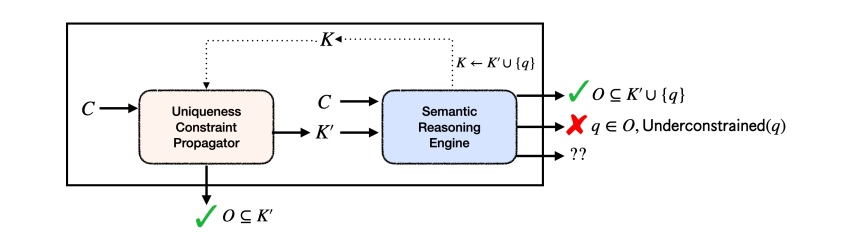
\includegraphics[width=180mm]{QED_algo.png}
\caption{Алгоритм работы метода $QED^2$}
\label{QED_algo}
\end{figure}

Инструмент принимает на вход $R1CS$ схему и пытается определить достаточно ли в ней ограничений. Результат работы инструмента может быть одним из следующих:

\begin{itemize}
    \item Ограничений достаточно. Это означает, что все скрытые переменные однозначно определяются входными, и инструмент смог это математически подтвердить.
    \item Ограничений недостаточно. В этом случае инструмент предоставит для конкретных входных значений два набора скрытых переменных, которые удовлетворяют схеме.
    \item Неопределённость. Инструмент не может дать точный ответ, так как SMT-solver не смог найти решение задачи за выделенное время.
\end{itemize}

Рассмотрим подробнее алгоритм работы инструмента, представленный на рисунке \ref{QED_algo}.

На вход алгоритму подаётся схема $C(I,W,O)$, где $I$ - входные переменные, $W$ - промежуточные, $O$ - выходные. $K$ - множество переменных, которые однозначно задаются входными данными, независимо от их значения. Изначально в $K$ лежат все входные переменные. По сути инструмент использует своеобразный метод абстрактной интерпретации - каждая переменная либо однозначно определена, тогда она лежит во множестве $K$, либо не определена. При этом во время работы метода поддерживается второе состояние абстрактной интерпретации - список возможных значений переменной. Изначально всем переменным присвоены все значения их поля $F_p$, то есть интервал $0..p-1$. Далее в цикле выполняются следующие два шага, цель каждого из которых - расширить множество $K$:

\begin{figure}[ht!]
    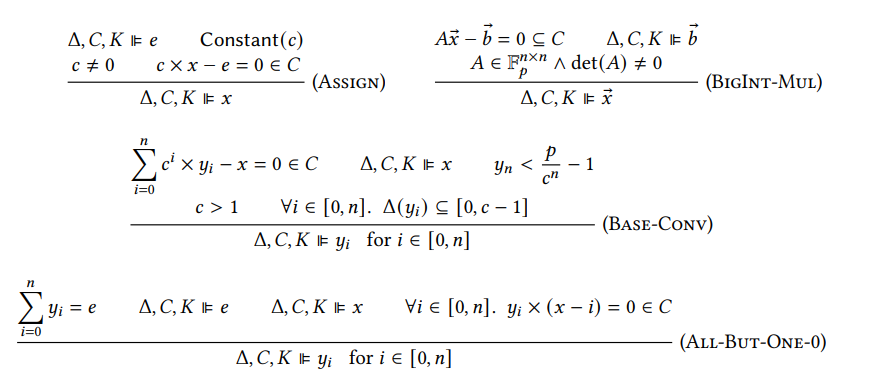
\includegraphics[width=180mm]{QED_rules.png}
    \caption{Правила вывода для абстрактной интерпретации определённости переменной}
    \label{QED_rules}
\end{figure}

\begin{figure}[ht!]
    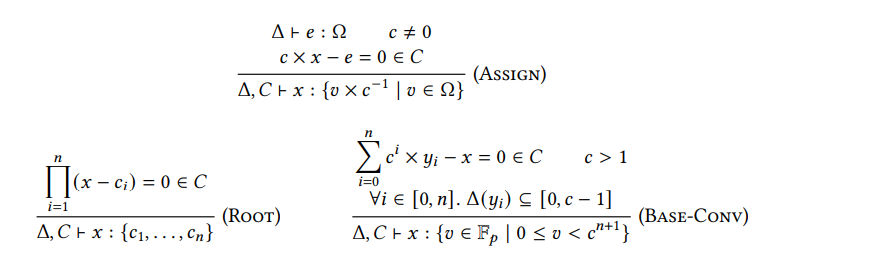
\includegraphics[width=180mm]{QED_values.png}
    \caption{Правила вывода для абстрактной интерпретации значений переменной}
    \label{QED_values}
\end{figure}

\begin{enumerate}
    \item Шаг распространения определённости на основе правил. На этом шаге используются особенности схемы арифметизации $R1CS$, а именно - 4 правила вывода, которые эффективно работают на схемах. Правила представлены на рисунке \ref{QED_rules}. Этот шаг работает до тех пор, пока какое-то из правил работает и в множество $K$ добавляются новые переменные. Если правила неприменимы, то инструмент переходит к следующему шагу. При это параллельно вычисляется абстрактная интерпретация значений переменных по правилам на рисунке \ref{QED_values}.
    \item Далее каждую из неопределённых переменных алгоритм пытается доопределить при помощи солвера. Для этого формируется вторая схема $C'$ - полная копия первой, кроме названий переменных. Чтобы добавить в формулу для солвера знания о переменных, накопленные на предыдущих шагах алгоритма, определяются две формулы:
    \begin{enumerate}
        \item $\phi = \land_{u \in K} (u = u')$ - формула сужает перебор - уже определённые переменные должны быть равны.
        \item - кодируем в формулу все имеющиеся абстрактные интерпретации значений для каждой из переменных.
    \end{enumerate}
    Итоговую формула отдаётся решателю CVC5\footnote[1]{\href{https://github.com/cvc5/cvc5}{https://github.com/cvc5/cvc5}}
\end{enumerate}


Среди схем, которые может решить $QED^2$, $QED^2$ возвращает результаты, подтвержденные для подавляющего большинства - $89\%$.
Этот результат ожидаем, поскольку многие схемы, входящие в состав circomlib-utils и circomlib-core, написаны криптографами, которые также являются экспертами Circom. Однако существует 13 схем, для
которых $QED^2$ выдает контрпримеры, что означает, что эти схемы доказуемо недостаточно ограничены.

\subsection{$Кorrekt^2$}

\subsection{Выводы}
\indent

Для fuzz-тестирования шаблонизаторов предлагается использовать наиболее отличившиеся идеи. Среди будущих мутаций обязательно должны присутствовать скрещивание и замена поддерева на случайное, потому что они выделяются среди остальных. Для генерации тестов можно использовать алгоритм построения похожих, вероятности вычислить по реальным программам. Для борьбы с семантическими ошибками можно использовать идеи из Grammarinator. Среди стратегий обработки тестов нет явно выделяющейся, но идеи, описанные в EvoGFuzz, мало изучены, предлагается исследовать именно их.

\newpage
\section{Результаты}
\indent

В рамках данной работы были получены следующие результаты:
\begin{itemize}
    \item Сделан обзор методов fuzz-тестирования программ, принимающих на вход данные, порождаемые КС-грамматикой. Выделены критерии для сравнения таких фаззеров.
    \item Произведён анализ существующих инструментов. На его основе предложен алгоритм для fuzz-тестирования шаблонизаторов.
\end{itemize}

\newpage

\begin{thebibliography}{}
    \addcontentsline{toc}{section}{Список литературы}
    \bibitem{litlink1}  PlonK: Permutations over Lagrange-bases for Oecumenical Noninteractive arguments of Knowledge [Электронный ресурс]. URL: \href{https://eprint.iacr.org/2019/953.pdf}{https://eprint.iacr.org/2019/953.pdf} (дата обращения: 26.05.2024)
    \bibitem{litlink2}  Automated Analysis of Halo2 Circuit [Электронный ресурс]. URL: \href{https://ceur-ws.org/Vol-3429/paper3.pdf}{https://ceur-ws.org/Vol-3429/paper3.pdf} (дата обращения: 26.05.2024)
    \bibitem{litlink3}  Certifying Zero-Knowledge Circuits with Refinement Types [Электронный ресурс]. URL: \href{https://eprint.iacr.org/2023/547.pdf}{https://eprint.iacr.org/2023/547.pdf} (дата обращения: 26.05.2024)
    \bibitem{litlink4}  SoK: What don’t we know? Understanding Security Vulnerabilities in SNARKs [Электронный ресурс]. URL: \href{https://arxiv.org/pdf/2402.15293}{https://arxiv.org/pdf/2402.15293} (дата обращения: 26.05.2024)
    \bibitem{litlink5}  Halo2 Book [Электронный ресурс]. 
    URL: \href{https://zcash.github.io/halo2/index.html}{https://zcash.github.io/halo2/index.html}
    (дата обращения: 26.05.2024)
    \bibitem{litlink6}  MoonMath manual [Электронный ресурс]. URL: \href{https://leastauthority.com/community-matters/moonmath-manual/}{https://leastauthority.com/community-matters/moonmath-manual/} (дата обращения: 26.05.2024)
    \bibitem{litlink7}  Automated Detection of Under-Constrained Circuits in Zero-Knowledge Proofs [Электронный ресурс]. URL: \href{https://eprint.iacr.org/2023/512.pdf}{https://eprint.iacr.org/2023/512.pdf} (дата обращения: 26.05.2024)
    \bibitem{litlink8}  Compositional Formal Verification
    of Zero-Knowledge Circuits [Электронный ресурс]. URL: \href{https://eprint.iacr.org/2023/1278.pdf}{https://eprint.iacr.org/2023/1278.pdf} (дата обращения: 26.05.2024)
    \bibitem{litlink9}  Formal Verification of Zero-Knowledge Circuits [Электронный ресурс]. URL: \href{https://arxiv.org/pdf/2311.08858}{https://arxiv.org/pdf/2311.08858}(дата обращения: 26.05.2024)
    \bibitem{litlink10}  Franklyn Wang (2022): Ecne: Automated Verification of ZK Circuits. OxPARC Blog [Электронный ресурс]. URL: \href{https://0xparc.org/blog/ecne}{https://0xparc.org/blog/ecne}(дата обращения: 26.05.2024)
    \bibitem{litlink11}  Plookup: A simplified polynomial protocol for
    lookup tables [Электронный ресурс]. URL: \href{https://eprint.iacr.org/2020/315.pdf}{https://eprint.iacr.org/2020/315.pdf}(дата обращения: 26.05.2024)
    \bibitem{litlink12}  ZERO-KNOWLEDGE ROLLUPS [Электронный ресурс]. URL: \href{https://ethereum.org/en/developers/docs/scaling/zk-rollups/}{https://ethereum.org/en/developers/docs/scaling/zk-rollups/}(дата обращения: 26.05.2024)
    \bibitem{litlink13}  Circom [Электронный ресурс]. URL: \href{https://docs.circom.io/}{https://docs.circom.io/}(дата обращения: 26.05.2024)
    \bibitem{litlink14}  Zokrates [Электронный ресурс]. URL: \href{https://zokrates.github.io/}{https://zokrates.github.io/}(дата обращения: 26.05.2024)
\end{thebibliography}

\end{document}